\ifdefined\isstandalone
\title{6.047/6.878 Lecture 21: Phylogenomics II {\tmabbr{}}}
\author{Guest Lecture by\\
  Matt Rasmussen \\
  Scribed by Jerry Wang and Dhruv Garg}
\maketitle
\chead{6.047/6.878 Lecture 21: Phylogenomics II}
\lhead{}
\rhead{}
{\pagebreak}
{\tableofcontents}
{\pagebreak}
{\listoffigures}
\else
\chapter{Phylogenomics II}
\author{Guest Lecture by\\
  Matt Rasmussen \\
  Scribed by Jerry Wang and Dhruv Garg}
\chead{6.047/6.878 Lecture 21: Phylogenomics II}
\lhead{} 
\rhead{} 
\minilof
\fi 
\pagestyle{fancy} 

\ifdefined\isstandalone
\def\@mydir{images} 
\fi
\ifdefined\ischapter
\def\@mydir{../Lecture21_Phylogenomics/images} 
\fi 
\ifdefined\ismaster
\def\@mydir{Lecture21_Phylogenomics/images} 
\fi 
% ####################################################################
\section{Introduction}

Guest lecturer Matt Rasmussen, a former student of Manolis’s presented
our secondphylogenomics lecture. The lecture finished explaining max
likelihood methods for phylogenetics,and then progressed to more
advanced uses of phylogenetics such as inferring orthologs, paralogs,
gene duplication and gene loss. This led to learning across gene trees
and modeling populations and allele frequencies.

In previous lectures, we studied various algorithms to obtain
phylogenetic species trees. Similar studies can be performed to study
phylogeny of gene families, or sets of orthologous and paralogous
genes. Given multiply aligned sequences, several techniques discussed
in previous lectures could be employed for constructing a gene tree,
including nearest neighbor joining, and hierarchical clustering. If in
addition to the aligned genes, we also have a species tree (which can
often be taken as a given for sufficiently diverged species), then we
should be able to formulate a consistent view of the evolutionary
process; namely, we hope to map the gene tree onto the species
tree. These mappings between the two trees are called
reconciliations. The standard phylogenomic pipeline can be summarized
as follows:

\begin{enumerate}
\item Blast protein sequences against each other to score similarities.
\item Use this metric to cluster genes into families of relatedness. 
\item Build multiple alignments. 
\item From the alignments, build gene trees. 
\item Reconcile the gene tree to the species tree. 
\end{enumerate} 

\subsection{Phylogenetics}
The two main pipe lines for building trees are distance-based and
character-based. Last lecture focused on distance-based pipeline. In
distance-based, you form a pair-wise distance matrix using
Jukes-Cantor or Kimura. Then use Neighbor Joining or UPGMA to
reconstruct a tree from the matrix. Distance based pipelines use a
fixed number of steps so and UPGMA and NJ have a running time is
$O(n^3)$. However, there are flaws to this approach. Distance-based
metrics are overly simplified and under measure the rate of mutation
because a nucleotide that gets mutated back to its original form is
counted as not mutated.

Today’s lecture focuses on the character-based pipeline, which is NP
Hard so we have to resort to heuristics. The basic idea is we want to
search through different trees and test each one. We start with an
initial tree, then compute the probability/likelihood, then explore
the tree space using methods such as nearest neighbor interchange
(NNI), compute the score again, loop and then return the tree with the
highest score as the answer. Using NNI, we can go to all trees in the
tree space. The problem is that the tree space is very big (why it is
NP hard).

\begin{figure}[ht!]
  \centering
  \scalebox{.3}{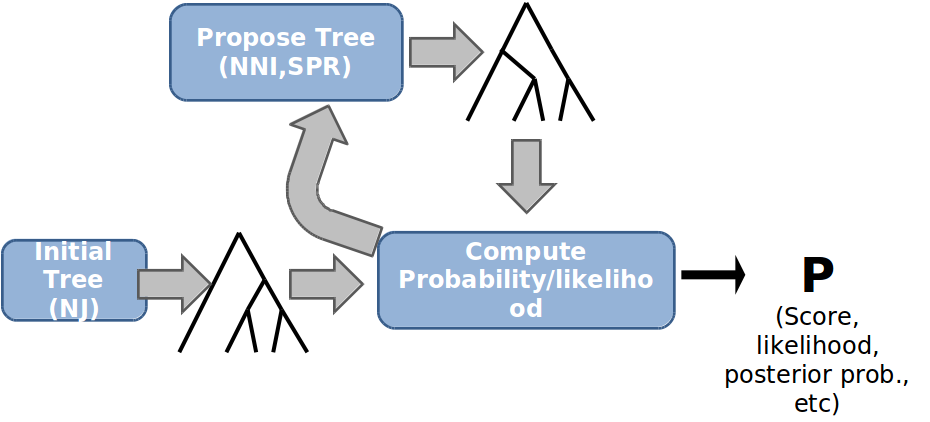
\includegraphics{\getdir/Fig01_HeuristicTreeSearch.png}}
  \caption{Heuristic tree search in character-based reconstruction}
  \label{Fig01_HeuristicTreeSearch}
\end{figure}

\noindent For the scoring metric, we want to maximize

\begin{figure}[ht!]
  \centering
  \scalebox{.3}{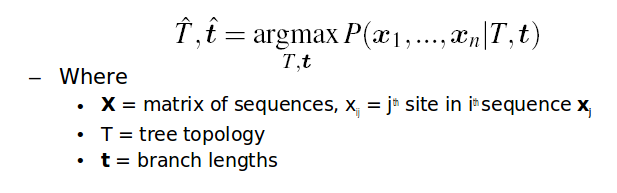
\includegraphics{\getdir/Fig02_MLScoringStep.png}}
  \caption{Scoring metric for heuristic tree search}
  \label{Fig02_MLScoringStep}
\end{figure}

Using the Felsenstein peeling algorithm, we can efficiently compute
$P(X|T,B)$ by buildign up a dynamic programming problem. We can first
look at site evolution along a single brance, then build on that and
look at sequence evolution and then look at site evolution along an
entire tree. Site evolution uses the Jukes-Cantor model and has the
definition

\begin{figure}[ht!]
  \centering
  \scalebox{.3}{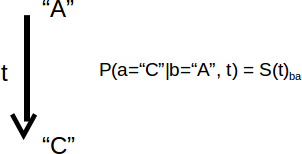
\includegraphics{\getdir/Fig03_SiteEvolution.png}}
  \caption{Site evolution uses the Jukes-Cantor model}
  \label{Fig03_SiteEvolution}
\end{figure}
\noindent If we assume site independence, sequence evolution is just
the product of site evolution:

\begin{figure}[ht!]
  \centering
  \scalebox{.3}{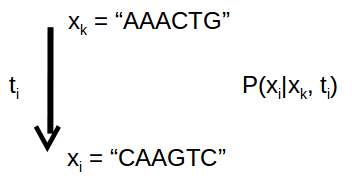
\includegraphics{\getdir/Fig04_SequenceEvolution.png}}
  \caption{Sequence evolution is the product of site evolution}
  \label{Fig04_SequenceEvolution}
\end{figure}

\noindent Assuming site independence does not always hold for example
in RNA coding r gions the sites is not independent due to RNA
folding. To move to sequence evolution over an entire tree, we assume
branch independence once we condition on the parent sequence.

\begin{figure}[ht!]
  \centering
  \scalebox{.3}{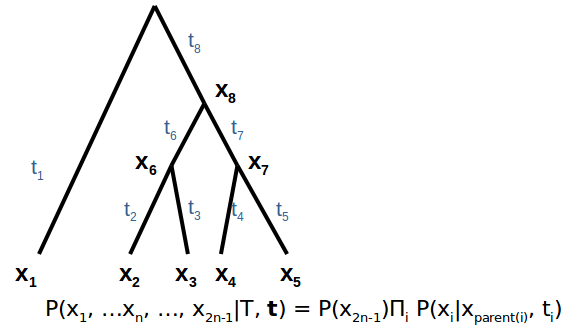
\includegraphics{\getdir/Fig05_SequenceEvolutionOverTree.png}}
  \caption{Sequence evolution over an entire tree.}
  \label{Fig05_SequenceEvolutionOverTree}
\end{figure}

\noindent From the equation in sequence evolution over an entire tree,
we need both internal nodes and leaves $(x_1,...x_{2n-1})$ but only
leaves $(x_1,...x_n)$ are given so we need to marginalize over
unknowns $(x_{n+1},...,x_{2n-1})$. Using a factorization trick:

$P(x_1,x_2,x_3,x_4|T,t)$ 
$= \Sigma x_5 \Sigma x_6 \Sigma x_7 P(x_1,x_2,x_3,x_4,x_5,x_6,x_7|T,t)$

$= \Sigma x_5 \Sigma x_6 \Sigma x_7 P(x_1|x_5,t_1)P(x_2|x_5,t_1)P(x_3|x_6,t_3)P(x_4|x_6,t_4)$ 

$= \Sigma x_7 P(x_7)$
$[\Sigma x_5 P(x_5|x_7,t_5)P(x_1|x_5,t_1)P(x_2|x_5,t_1)]$
$[\Sigma x_6 P(x_6|x_7,t_6)P(x_3|x_6,t_3)P(x_4|x_6,t_4)]$

\noindent The Peeling algorithm builds a DP table. Each entry contains
the probability of seeing the leaf data below node I, give that node I
has base a at site j. The leaves of the table are initialized based on
the observed sequence. Entries are populated in post-order
traversal. The runtime of the Peeling algorithm is $O(nmk^2)$.

\begin{figure}[ht!]
  \centering
  \scalebox{.3}{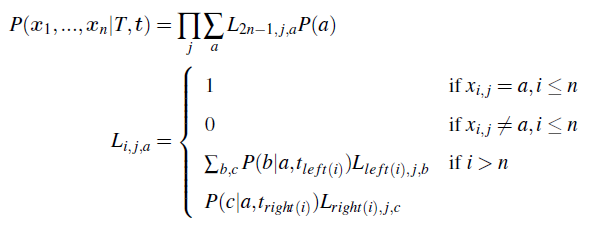
\includegraphics{\getdir/Fig06_PeelingAlgorithm.png}}
  \caption{Peeling Algorithm}
  \label{Fig06_PeelingAlgorithm}
\end{figure}

\noindent The Peeling algorithm scores one tree and we need to use the
search algorithm to search for more trees. The runtime is for one tree
while the entire runtime depends on how many trees you want to look
at.

\section{Inferring Orthologs/Paralogs, Gene Duplication and Loss}

\noindent There are two commonly used trees. The species tree uses
morphological characters, fossil evidence, etc to create a tree of how
species are related (leaves are species). Gene trees look at specific
genes in different species (leaves are genes).

\begin{figure}[ht!]
  \centering
  \scalebox{.3}{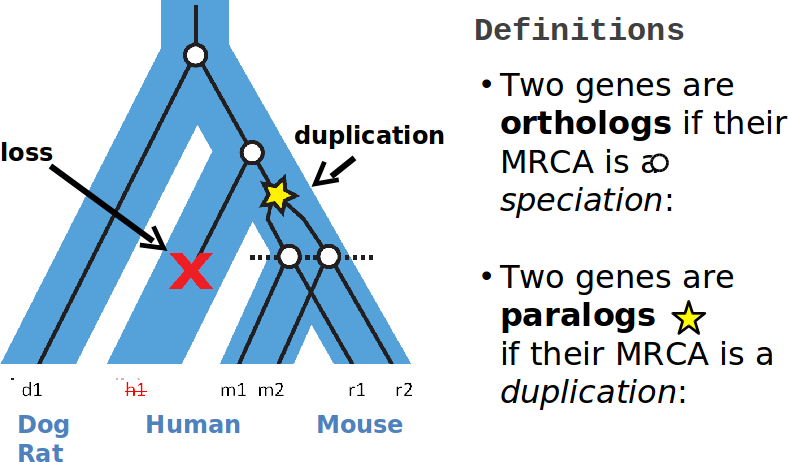
\includegraphics{\getdir/Fig07_GeneFamilyEvolution.png}}
  \caption{Gene Family Evolution: Gene Trees and Species Trees}
  \label{Fig07_GeneFamilyEvolution}
\end{figure}

\noindent Reconciliation is an algorithm to figure out how the gene tree fits inside  he species tree. It maps the vertices in the gene tree to vertices in the species tree. 

\begin{figure}[ht!]
  \centering
  \scalebox{.3}{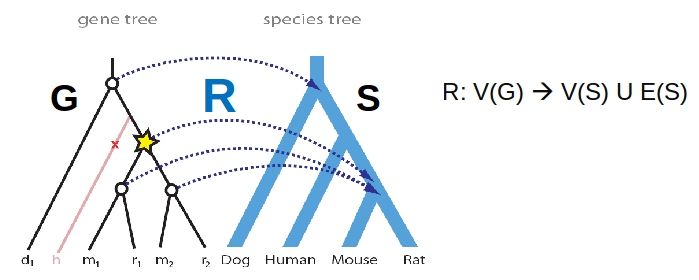
\includegraphics{\getdir/Fig08_MaximumParsimonyReconciliation.png}}
  \caption{Maximum Parsimony Reconciliation (MPR) } 
  \label{Fig08_MaximumParsimonyReconciliation}
\end{figure}

\noindent We want to minimize the duplication/loss so we want to map
events as low in the tree as possible to when they happened to
minimize loss.

\begin{figure}[ht!]
  \centering
  \scalebox{.3}{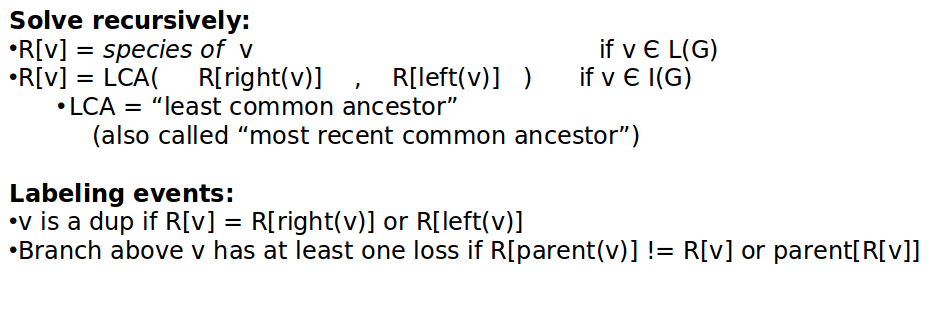
\includegraphics{\getdir/Fig09_MPRAlgorithm.png}}
  \caption{Maximum Parsimony Reconciliation Recursive Algorithm} 
  \label{Fig09_MPRAlgorithm}
\end{figure}

Duplication events map to the same as both of its children. Loss event
maps to gap in the mapping. Gene tree accuracy is important; even one
branch misplaced can dramatically increases error.

\section{Learning Across Gene Trees}

\begin{figure}[ht!]
  \centering
  \scalebox{.3}{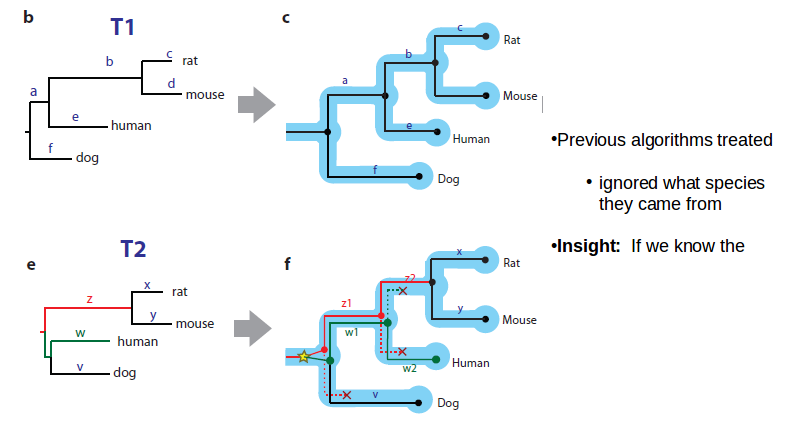
\includegraphics{\getdir/Fig10_LearningAcrossGeneTrees.png}}
  \caption{Using species trees to improve gene tree reconstruction.} 
  \label{Fig10_LearningAcrossGeneTrees}
\end{figure}

If we knew the species tree we could know beforehand that we expect
the branch to be longer. We can develop a model for what kind of
branch lengths we can expect. We can use conserved gene order to tell
orthologs and build trees.

\begin{figure}[ht!]
  \centering
  \scalebox{.3}{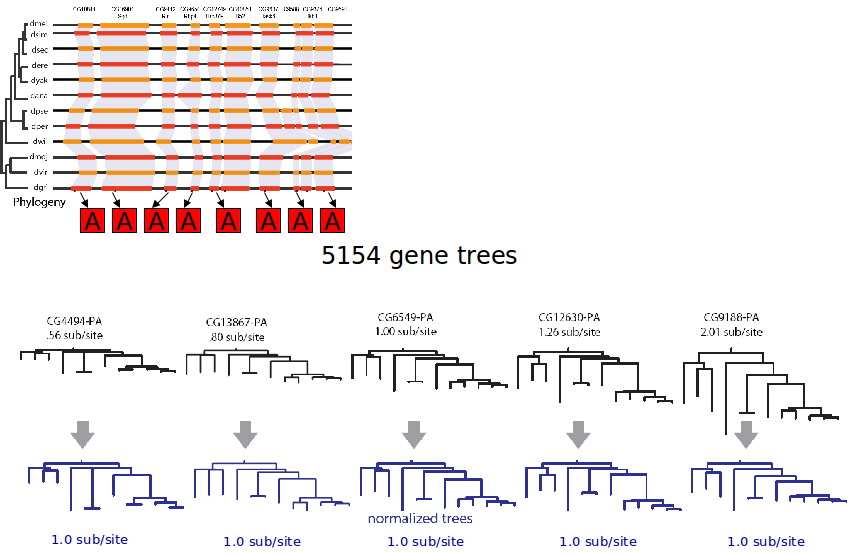
\includegraphics{\getdir/Fig11_DevelopingRatesModel.png}}
  \caption{We can develop a model for what kind of branch lengths we
    can expect. We can use conserved gene order to tell orthologs and
    build trees.}
  \label{Fig11_DevelopingRatesModel}
\end{figure}

When gene is fast evolving in one species, it is fast evolving in all
species. We can model a branch length as two different rate
components. One is gene specific(present across all species) and a
species specific which is customized to a specific species.

\begin{figure} [ht!] 
  \centering
  \scalebox{.3}{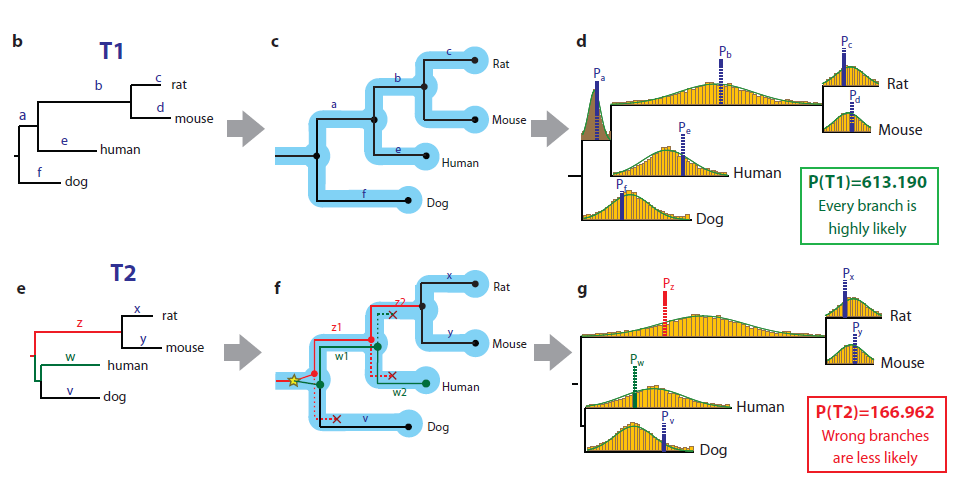
\includegraphics{\getdir/Fig12_UsingRateModels.png}}
  \caption{Branch length can be modeled as two different rate
    components: gene specific and species specific.}
  \label{Fig12_UsingRateModels}
\end{figure} 

\noindent This method greatly improves reconstruction accuracy.

\section{Modeling Population and Allele Frequencies}
People keep sequencing genomes so looking at how populations evolve is
becoming more and more important and feasible. The Wright-fisher model
is used to study drifts, bottlenecks, etc. The coalescent model
combines the Wright-fisher with trees. Wright-fisher was designed to
study the effect of finite population sizes. We need to assume
population size is fixed at $N$, random mating, non-overlapping
generations.

\begin{figure} [ht!] 
  \centering 
  \scalebox{.3}{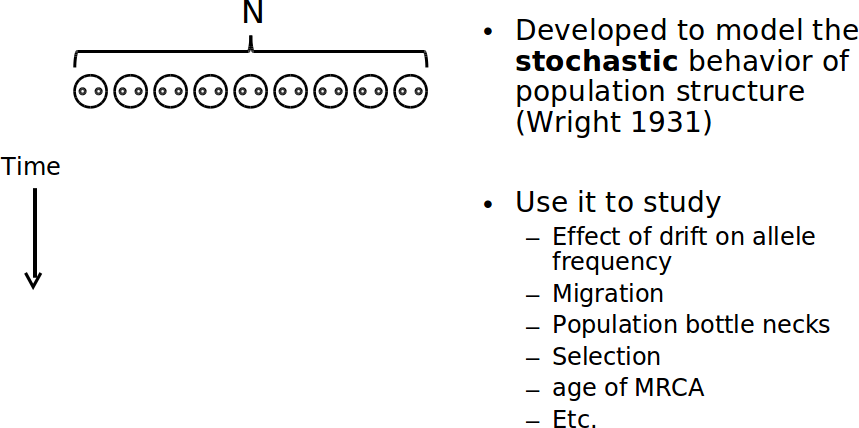
\includegraphics{\getdir/Fig13_FisherWrightModel.png}}
  \caption{The Wright-Fisher model}
  \label{Fig13_FisherWrightModel}
\end{figure} 

\noindent Continue for many generations and ignore ordering of chromosomes.

\begin{figure} [ht!] 
  \centering 
  \scalebox{.3}{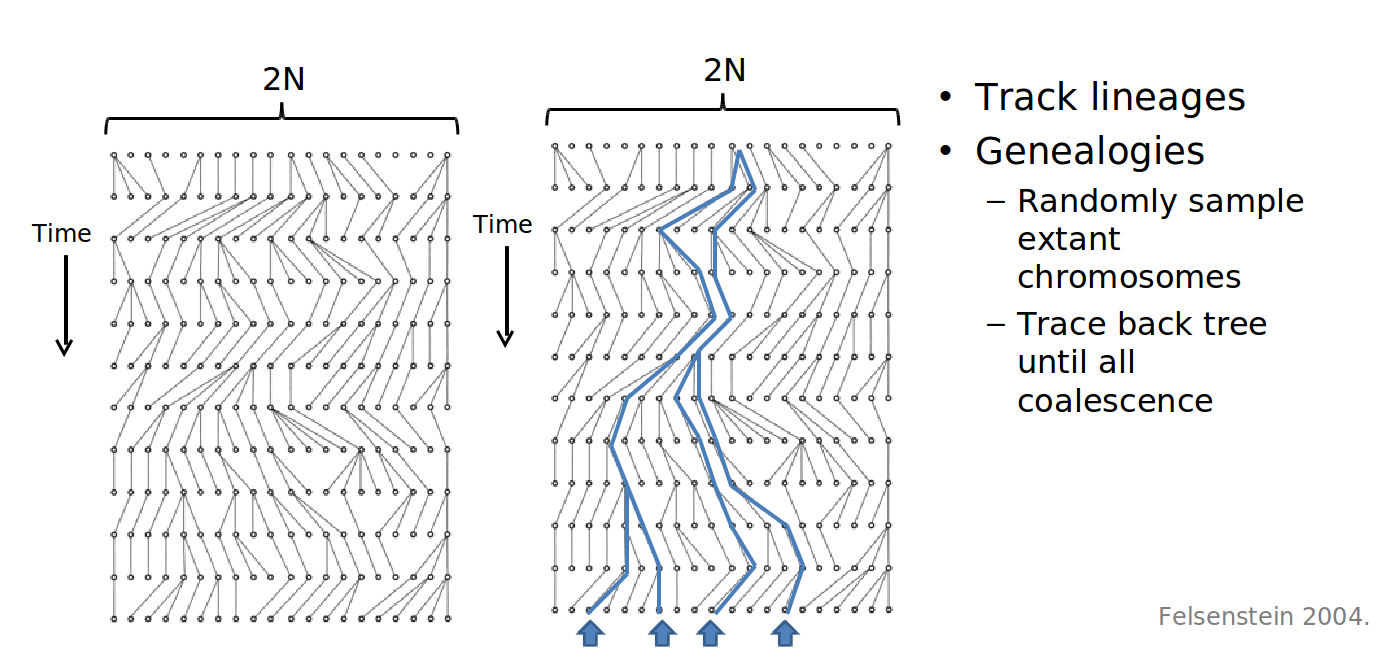
\includegraphics{\getdir/Fig14_FisherWrightManyGenerations.png}}
  \caption{The Wright-Fisher model continued over many generations and
    ignoring the ordering of chromosomes.}
  \label{Fig14_FisherWrightManyGenerations}
\end{figure} 

The coalescent model only focuses on the genealogy. It only is
concerned about the lineages we have sequences for; do not have to
worry about others. It is a probabilistic model that works backwards
in time to find when they have common ancestors.

\begin{figure} [ht!] 
  \centering 
  \scalebox{.3}{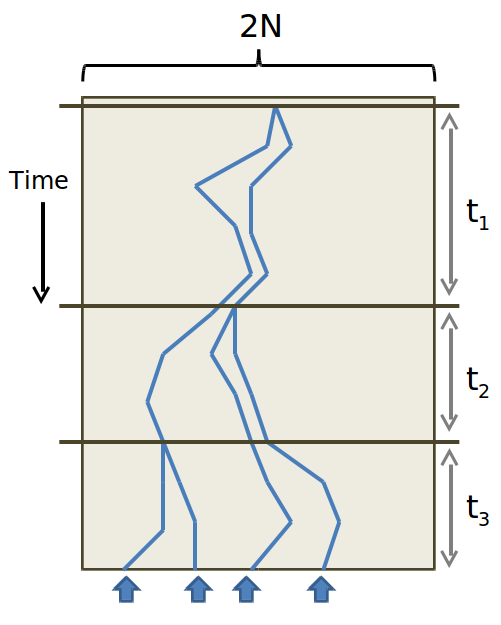
\includegraphics{\getdir/Fig15_CoalescentModel.png}}
  \caption{The coalescent model.}
  \label{Fig15_CoalescentModel}
\end{figure} 

Say we have $2N$ individuals, what is the probability that k lineages
do not have any coalescent events in parental generation? What is the
probability that the first coalescent of $k$ lineages is at $t$
generations? This process can be seen as a geometric distribution.

\begin{figure} [ht!] 
  \centering 
  \scalebox{.3}{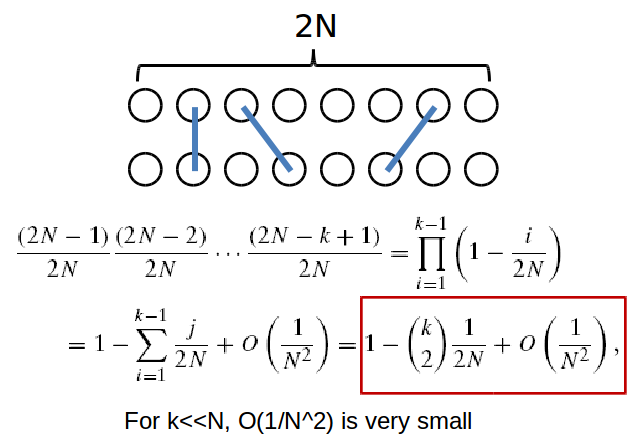
\includegraphics{\getdir/Fig16_CoalescentProbDist.png}}
  \caption{Geometric probability distribution for coalescent events in k lineages.}
  \label{Fig16_CoalescentProbDist}
\end{figure} 

\noindent Can repeat to find when all individuals coalesce. Each
branch of species tree can be seen as having its own Wright-Fisher
inside of it.

\begin{figure} [ht!] 
  \centering 
  \scalebox{.3}{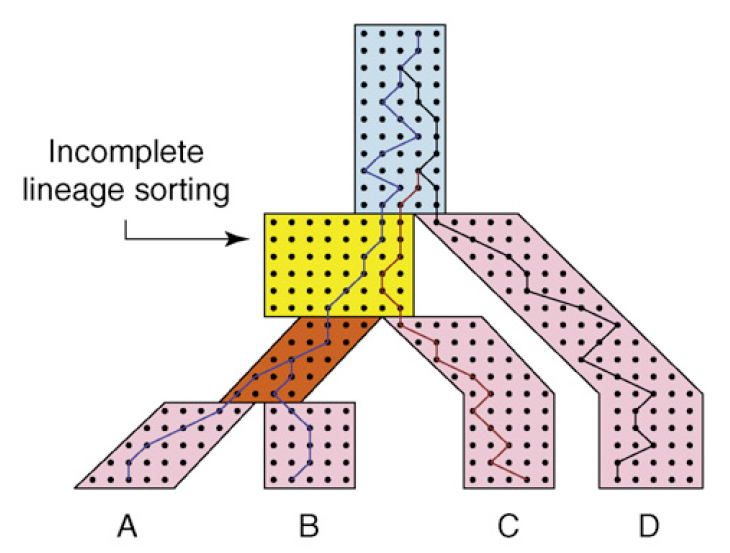
\includegraphics{\getdir/Fig17_MultispeciesCoalescent.png}}
  \caption{Multispecies Coalescent Model. Leaf branches track one
    lineage. There is a lag time from when population separated and
    when two actual gene lineages find a common ancestor. The rate of
    coalescent slows down as N gets bigger and for short
    branches. Deep coalescent is depicted in light blue for three
    lineages. The species and gene tree are incongruent since C and D
    are sisters in gene tree but not the species tree. There is a
    $\frac{2}{3}$ chance that incongruence will occur because once we
    get to the light blue section, the Wright-fisher is memory less
    and there is only $\frac{1}{3}$ chance that it will be
    congruent. Effect of incongruence is called incomplete lineage
    sorting.}
  \label{Fig17_MultispeciesCoalescent}
\end{figure} 

\section{SPIDIR:Background} 
As presented in the supplementary information for SPIDIR, a gene
family is the set of genes that are descendents of a single gene in
the most recent common ancestor (MRCA) of all species under
consideration. Furthermore, genetic sequences undergo evolution at
multiple scales, namely at the level of base pairs, and at the level
of genes. In the context of this lecture, two genes are orthologs if
their MRCA is a speciation event; two genes are paralogs if their MRCA
is a duplication event.

In the genomic era, the species of a modern genes is often known;
ancestral genes can be inferred by reconciling gene- and
species-trees. A reconciliation maps every gene-tree node to a
species-tree node. A common technique is to perform Maximum Parsimony
Reconciliation (MPR), which finds the reconciliation R implying the
fewest number of duplications or losses using the recursion over inner
nodes $v$ of a gene tree $G$. MPR fist maps each leaf of the gene tree
to the corresponding species leaf of the species tree. Then the
internal nodes of $G$ are mapped recursively:

$R(v) = MRCA(R(right(v)),R(left(v)))$

\noindent If a speciation event and its ancestral node are mapped to the same node on the species tree. Then the ancestral node must be an duplication event.

Using MPR, the accuracy of the gene tree is crucial. Suboptimal gene
trees may lead to an excess of loss and duplication events. For
example, if just one branch is misplaced (as in
\ref{Fig02_MLScoringStep}) then reconciliation infers 3 losses and 1
duplication event. In \cite{Rasmussen}, the authors show that the
contemporaneous current gene tree methods perform poorly (60\%
accuracy) on single genes. But if we have longer concatenated genes,
then accuracy may go up towards 100\%. Furthermore, very quickly or
slowly evolving genes carry less information as compared with
moderately diverging sequences (40-50\% sequence identity), and
perform correspondingly worse. As corroborated by simulations, single
genes lack sufficient information to reproduce the correct species
tree. Average genes are too short and contains too few
phylogenetically informative characters. While many early gene tree
construction algorithms ignored species information, algorithms like
SPIDIR capitalize on the insight that the species tree can provide
additional information which can be leveraged for gene tree
construction. Synteny can be used to independently test the relative
accuracy of different gene tree reconstructions. This is because
syntenic blocks are regions of the genome where recently diverged
organisms have the same gene order, and contain much more information
than single genes.

\begin{figure} [ht!] 
  \centering 
  \scalebox{.3}{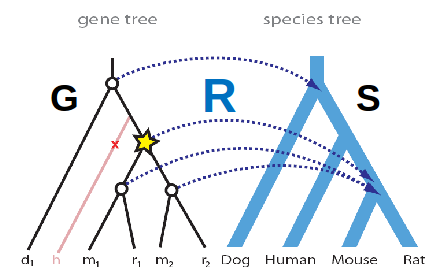
\includegraphics{\getdir/Fig18_AlternateReconciliations.png}}
  \caption{MPR reconciliation of genes and species tree.}
  \label{Fig18_AlternateReconciliations}
\end{figure} 

\begin{figure} [ht!] 
  \centering 
  \scalebox{.3}{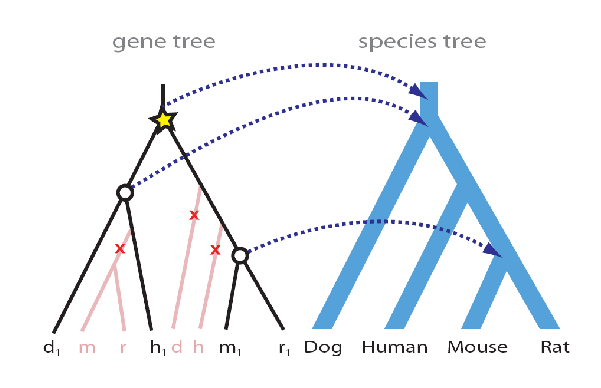
\includegraphics{\getdir/Fig19_GeneTreeInaccuracies.png}}
  \caption{Inaccuracies in gene tree.}
  \label{Fig19_GeneTreeInaccuracies}
\end{figure} 

There have been a number of recent phylogenomic algorithms including:
RIO \cite{Zmasek}, which uses neighbor joining (NJ) and bootstrapping
to deal with incogruencies, Orthostrapper \cite{Storm}, which uses NJ
and reconciles to a vague species tree, TreeFAM \cite{Li}, which uses
human curation of gene trees as well as many others. A number of
algorithms take a more similar track to SPIDIR \cite{Rasmussen},
including \cite{Arvestad}, a probabilistic reconciliation algorithm
\cite{Hollich}, a Bayesian method with a clock,\cite{Wapinski},and
parsimony method using species tree , as well as more recent
developments: \cite{Akerborg} a Bayesian method with relaxed clock and
\cite{Rasmussen2011}, a Bayesian method with gene and species specific
relaxed rates (an extension to SPIDIR) .

\section{SPIDIR: Method and Model} 
SPIDIR exemplifies an iterative algorithm for gene tree construction
using the species tree. In SPIDIR, the authors define a generative
model for gene-tree evolution. This consists of a prior for gene-tree
topology and branch lengths. SPIDIR uses a birth and death process to
model duplications and losses (which informs the prior on topology)
and then then learns gene-specific and species-specific substitution
rates (which inform the prior on branch lengths). SPIDIR is a
\textit{Maximum a posteriori (MAP)} method, and, as such, enjoys
several nice optimality criteria.

In terms of the estimation problem, the full SPIDIR model appears as
follows:

$argmax L,T,R P(L,T,R|D,S,\Theta) = argmax L,T,R P(D|T,L)P(L|T,R,S,\Theta)P(T,R|S,\Theta)$ 

The parameters in the above equation are: $D$ = alignment data , $L$ =
branch length $T$ = gene tree topology , $R$ = reconciliation , $S$ =
species tree (expressed in times) , $\Theta$ = ( gene and species
specific parameters [estimated using EM training], $\lambda$, $\mu$
dup/loss parameters)). This model can be understood through the three
terms in the right hand expression, namely:

\begin{enumerate} 
\item the sequence model-- $P(D|T,L)$. The authors used the common HKY
  model for sequence substitutions, which unifies Kimura's two
  parameter model for transitions and transversions with Felsenstein's
  model where substitution rate depends upon nucleotide equilibrium
  frequency.
\item the first prior term, for the rates model-- $P(L|T,R,S,\Theta)$,
  which the authors compute numerically after learning species and
  gene specific rates.
\item the second prior term, for the duplication/loss model--
  $P(T,R|S,\Theta)$, which the authors describe using a birth and
  death process.
\end{enumerate} 

Having a rates model is very rates model very useful, since mutation
rates are quite variable across genes. In the lecture, we saw how
rates were well described by a decomposition into gene and species
specific rates. In lecture we saw that an inverse gamma distribution
appears to parametrize the gene specific substitution rates, and we
were told that a gamma distribution apparently captures species
specific substitution rates. Accounting for gene and species specific
rates allows SPIDIR to build gene trees more accurately than previous
methods. A training set for learning rate parameters can be chosen
from gene trees which are congruent to the species tree. An important
algorithmic concern for gene tree reconstructions is devising a fast
tree search method. In lecture, we saw how the tree search could be
sped up by only computing the full $argmax L,T,R P(L,T,R|D,S,\Theta)$
for trees with high prior probabilites. This is accomplished through a
computational pipeline where in each iteration 100s of trees are
proposed by some heuristic. The topology prior $P(T,R|D,S,\Theta)$ can
be computed quickly. This is used as a filter where only the
topologies with high prior probabilities are selected as candidates
for the full likelihood computation.

\noindent The performance of SPIDIR was tested on a real dataset of 21
fungi. SPIDER recovered over 96\% of the synteny orthologs while other
algorithms found less than 65\%. As a result, SPIDER invoked much
fewer number of duplications and losses.

\section{Conclusion} 
Incorporating species tree information into the gene tree building
process via introducing separate gene and species substitution rates
allows for accurate parsimonious gene tree reconstructions. Previous
gene tree reconstructions probably vastly overestimated the number of
duplication and loss events. Reconstructing gene trees for large
families remains a challenging problem.

\section{Current Research Directions}
\section{Further Reading}
\section{Tools and Techniques} 
\section{What Have We Learned?}

\nocite{*}
\bibliographystyle{plain}
\bibliography{Lecture21_Phylogenomics} 
